\documentclass[a4paper,12pt]{article}
\usepackage[T2A]{fontenc} 
\usepackage[utf8]{inputenc}
\usepackage[english,russian]{babel} %орфография
\usepackage{circuitikz} % рисовать схемы (резисторы)
\usepackage{wrapfig} %картинка сбоку от текста
\usepackage{makecell} % 
\usepackage{tabularx} % кручу таблицы
\usepackage{graphicx} % графика
\usepackage{float} %
\usepackage{gensymb} % доп символы
\usepackage{cancel} %cancel symbol (зачеркивание)
\usepackage{amsmath,amsfonts,amssymb,amsthm,mathtools} % красивые буквы

%tikz (draw)

\usepackage{tikz} % рисование 

%tikz libraries

\usetikzlibrary{intersections} 
\usetikzlibrary{arrows.meta}
\usetikzlibrary{calc,angles,positioning}



\parindent=0ex % красная строка (ее отсутсвие)





\graphicspath{ {C:/Users/Admin/Documents/TEX/test} }

\newcommand{\R}{{\mathbb R}}
\newcommand{\N}{{\mathbb N}}
\newcommand{\fancy}[1]{{\mathbb{#1}}}
\DeclareMathOperator{\sgn}{sgn}
\newcommand{\uni}{\cup}
\newcommand{\inter}{\cap}

\begin{document}
	\begin{titlepage}
	\begin{center}
		МОСКОВСКИЙ ГОСУДАРСТВЕННЫЙ УНИВЕРСИТЕТ \\
		ИМ. М.В. ЛОМОНОСОВА \\
		
		
		\hfill \break
		Факультет вычислительной математики и кибернетики\\
		\vspace{2.5cm}
		\large{\textbf{Отчет по заданию № 1}}\\
		\hfill \break
		\\
	\end{center}
	
	\begin{flushright}
		Автор:\\
		Студент гр. 106\\
		Кондрашов Д.С.
	\end{flushright}
	
	\vspace{7cm}
	
	\begin{center}
		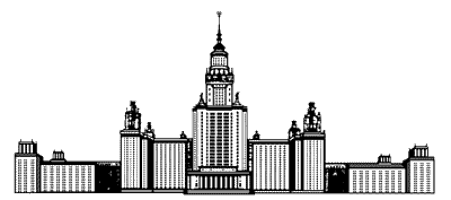
\includegraphics[width=0.3\linewidth]{msu_logo}
	\end{center}
	
	
	
	
	\vfill
	
	\begin{center} Москва, 2024 \end{center}
	
	\thispagestyle{empty}
	
\end{titlepage}
	\newpage
	\pagenumbering{arabic}
	
	\tableofcontents %оглавление
	\section*{дебильное название} % * - пропуск нумерации
	\section{title1}	
	\subsection{title2}
	\subsubsection{title3}
	\paragraph{title4}
	\begin{equation}		
		\int 3x^2dx
		\label {eq 1}
	\end{equation}
	\[
	\int 4x^2 dx
	\]
	\eqref{eq 2}
	\begin{eqnarray}
		x = x \\ \label{eq 2} \\
		x = z \\
		z = u  
	\end{eqnarray}
	\eqref{eq 2}
	\begin{figure}[H]
		\centering
		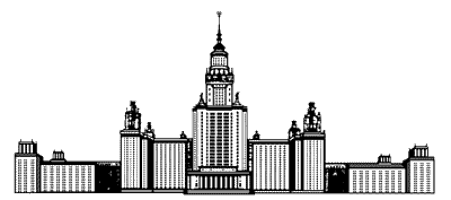
\includegraphics[width=0.7\linewidth]{msu_logo}
		\caption{}
		\label{fig:msulogo}
	\end{figure}
	\begin{figure} [H]
		\begin{tabular}{|c|c|c|c|cllllll}
			\hline
			4 & 4 & 1 & 5 & 7 & 3& & &3 & & 6 \\
			\hline
			1 & 0 & 0 & 0 & 1 & & & & & & \\
			\hline
			& 0 & 0 & 1 &  & & & & & & \\
			\hline& & & & & & & & & & 
		\end{tabular}
		\centering
	\end{figure}
	\textit{\textbf{бла бла бла}}
	
	
	
\end{document}